


%%% Introduction: 
% Why iterative solvers for large sparse systems of equations?


% \begin{frame}[fragile]{Iterative Solvers and Accelerators}
% 
%  \begin{block}{Iterative Solvers}
%    \begin{itemize}
%     \item Matrix-vector products and vector operations only
%     \item Expose more fine-grained parallelism
%     \item Preconditioners often desirable
%    \end{itemize}
%  \end{block}
% 
%  \begin{block}{Accelerators}
%    \begin{itemize}
%     \item Graphics processing units (GPUs)
%     \item Intel Xeon Phi
%    \end{itemize}
%  \end{block}
% 
%   \begin{center}
%    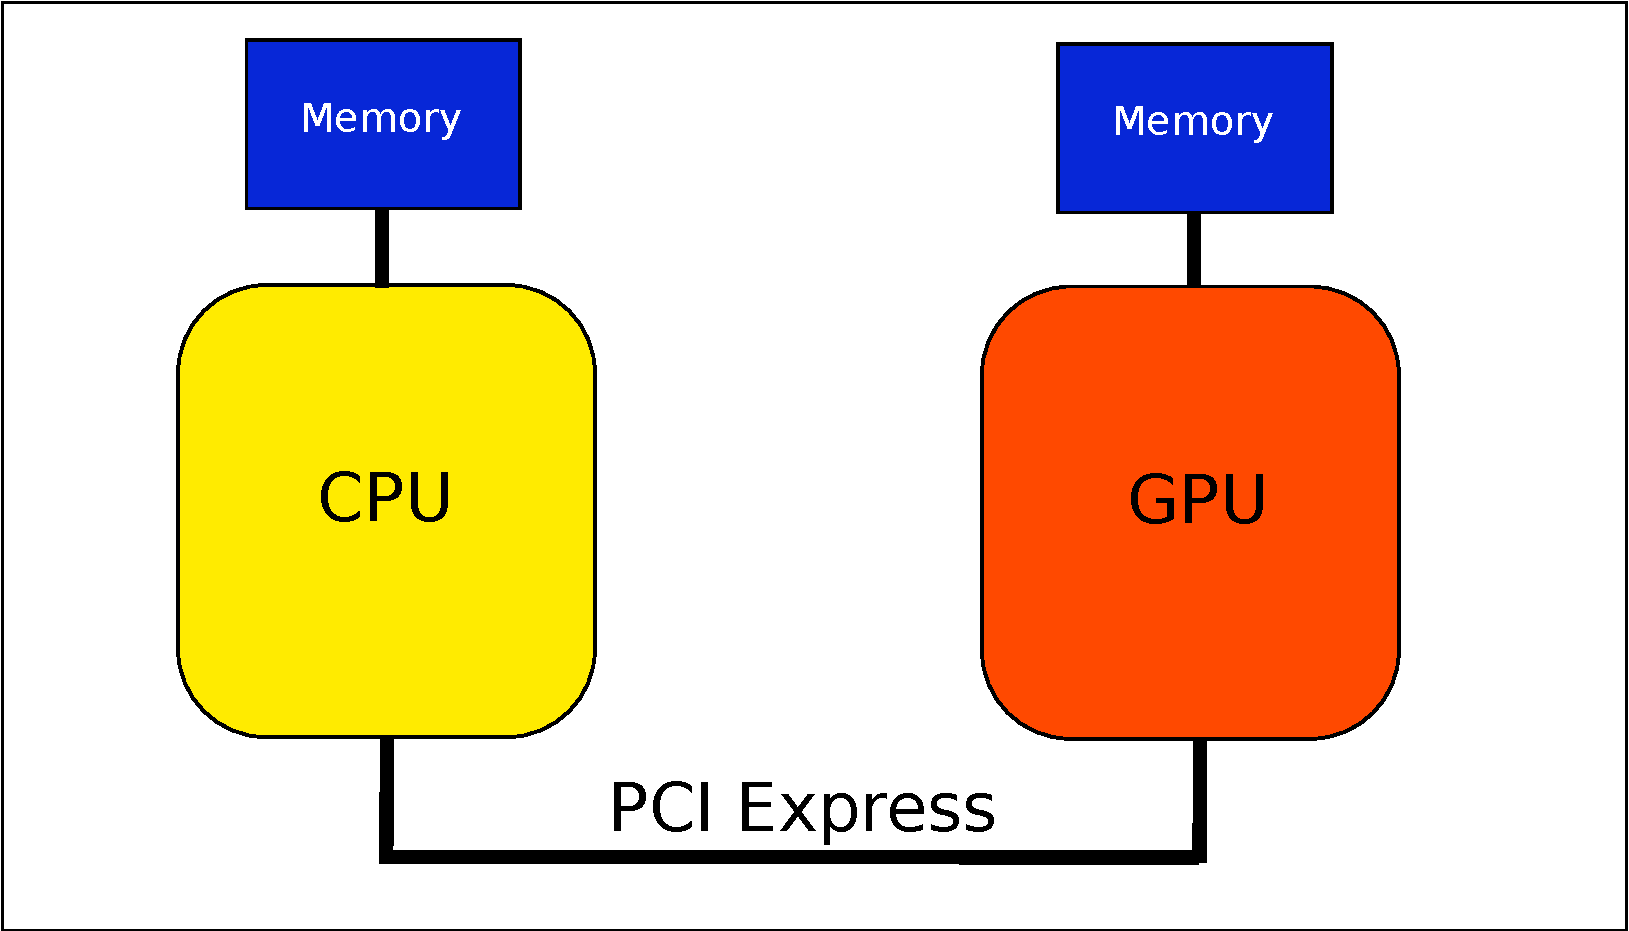
\includegraphics[width=0.6\textwidth]{figures/cpu-gpu-coarse}
%   \end{center}
% 
% \end{frame}



% Show CG algorithm <-> BLAS
\begin{frame}[fragile]{Conjugate Gradients}

 \begin{block}{}
  
   \begin{minipage}{0.45\textwidth}
      {\large \textbf{Pseudocode}} \\
      
      Choose $x_0$ \\
      $p_0 = r_0 = b - Ax_0$ \\
      For $i=0$ until convergence
     \begin{enumerate}
      \item Compute and store $Ap_i$
      \item Compute $\langle p_i, Ap_i \rangle$
      \item $\alpha_i = \langle r_i, r_i \rangle / \langle p_i, Ap_i \rangle$
      \item $x_{i+1} = x_{i} + \alpha_i p_i$          
      \item $r_{i+1} = r_i - \alpha_i Ap_i$       
      \item Compute $\langle r_{i+1}, r_{i+1} \rangle$
      \item $\beta_i = \langle r_{i+1}, r_{i+1} \rangle / \langle r_i, r_i \rangle$
      \item $p_{i+1} = r_{i+1} + \beta_i p_i$
     \end{enumerate}
     EndFor
   \end{minipage}
   \begin{minipage}{0.48\textwidth}
      {\large \textbf{BLAS-based Implementation}} \\
      
            - \\
      SpMV, AXPY \\
      For $i=0$ until convergence
     \begin{enumerate}
      \item SpMV
      \item DOT
      \item -
      \item AXPY         
      \item AXPY
      \item DOT
      \item -
      \item AXPY
     \end{enumerate}
     EndFor
   \end{minipage}
   
   \end{block}
   
\end{frame}


\begin{frame}[fragile]{Conjugate Gradients}

 \begin{block}{}
  
   \begin{minipage}{0.45\textwidth}
      {\large \textbf{Pseudocode}} \\
      
      Choose $x_0$ \\
      $p_0 = r_0 = b - Ax_0$ \\
      For $i=0$ until convergence
     \begin{enumerate}
      \item Compute and store $Ap_i$
      \item Compute $\langle p_i, Ap_i \rangle$
      \item $\alpha_i = \langle r_i, r_i \rangle / \langle p_i, Ap_i \rangle$
      \item $x_{i+1} = x_{i} + \alpha_i p_i$          
      \item $r_{i+1} = r_i - \alpha_i Ap_i$       
      \item Compute $\langle r_{i+1}, r_{i+1} \rangle$
      \item $\beta_i = \langle r_{i+1}, r_{i+1} \rangle / \langle r_i, r_i \rangle$
      \item $p_{i+1} = r_{i+1} + \beta_i p_i$
     \end{enumerate}
     EndFor
   \end{minipage}
   \begin{minipage}{0.48\textwidth}
      {\large \textbf{BLAS-based Implementation}} \\
      
            - \\
      SpMV, AXPY \\
      For $i=0$ until convergence
     \begin{enumerate}
      \item SpMV
      \item DOT {\color{red} $\leftarrow$ Global sync!}
      \item -
      \item AXPY         
      \item AXPY
      \item DOT {\color{red} $\leftarrow$ Global sync!}
      \item -
      \item AXPY
     \end{enumerate}
     EndFor
   \end{minipage}
   
   \end{block}
   
\end{frame}


\begin{frame}[fragile]{Conjugate Gradients}

 \begin{block}{}
  
   \begin{minipage}{0.45\textwidth}
      {\large \textbf{Pseudocode}} \\
      
      Choose $x_0$ \\
      $p_0 = r_0 = b - Ax_0$ \\
      For $i=0$ until convergence
     \begin{enumerate}
      \item Compute and store $Ap_i$
      \item Compute $\langle p_i, Ap_i \rangle$
      \item $\alpha_i = \langle r_i, r_i \rangle / \langle p_i, Ap_i \rangle$
      \item $x_{i+1} = x_{i} + \alpha_i p_i$          
      \item $r_{i+1} = r_i - \alpha_i Ap_i$       
      \item Compute $\langle r_{i+1}, r_{i+1} \rangle$
      \item $\beta_i = \langle r_{i+1}, r_{i+1} \rangle / \langle r_i, r_i \rangle$
      \item $p_{i+1} = r_{i+1} + \beta_i p_i$
     \end{enumerate}
     EndFor
   \end{minipage}
   \begin{minipage}{0.48\textwidth}
      {\large \textbf{BLAS-based Implementation}} \\
      
            - \\
      SpMV, AXPY \\
      For $i=0$ until convergence
     \begin{enumerate}
      \item SpMV {\color{blue} $\leftarrow$ No caching of $Ap_i$}
      \item DOT {\color{red} $\leftarrow$ Global sync!}
      \item -
      \item AXPY         
      \item AXPY  {\color{blue} $\leftarrow$ No caching of $r_{i+1}$}
      \item DOT {\color{red} $\leftarrow$ Global sync!}
      \item -
      \item AXPY
     \end{enumerate}
     EndFor
   \end{minipage}
   
   \end{block}
   
\end{frame}

\begin{frame}[fragile]{Conjugate Gradients}

 \begin{block}{}
 
 \begin{center}
  \vspace*{-0.5cm}
  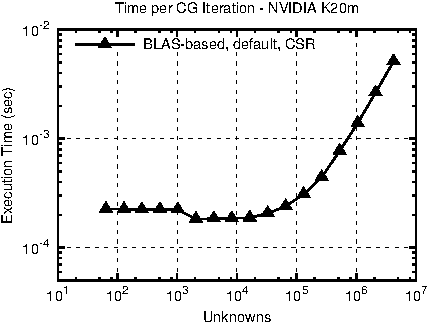
\includegraphics[width=0.85\textwidth]{figures/cg-k20m-0}
 \end{center}

 \begin{itemize}
  \item   \vspace*{-0.3cm} {\small (2D Finite Difference Discretization)}
 \end{itemize}

 \end{block}
   
\end{frame}

%%%%%%%%

% We ignore preconditioners here
% Show AMG scaling picture

\begin{frame}[fragile]{Conjugate Gradient}

 \begin{block}{Implications}
   \begin{itemize}
   \item Kernel launches expensive
   \item Delicate balance for preconditioners
  \end{itemize}
  
  \vspace*{6.1cm}
  \end{block}
   
\end{frame}

\begin{frame}[fragile]{Conjugate Gradient}

 \begin{block}{Implications}
   \begin{itemize}
   \item Kernel launches expensive
   \item Delicate balance for preconditioners
  \end{itemize}
  
  \begin{center}
   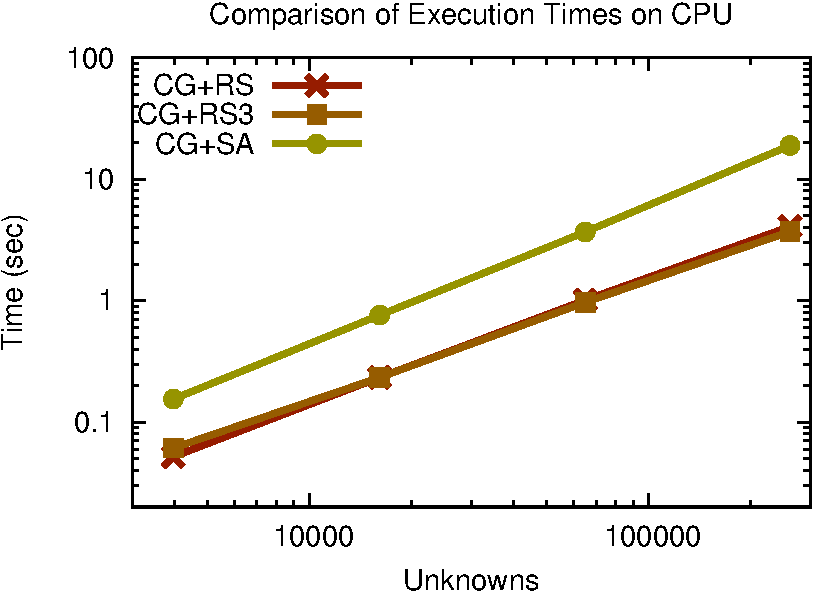
\includegraphics[width=0.7\textwidth]{figures/cpu_scaling-1}
  \end{center}
 \end{block}
   
\end{frame}


\begin{frame}[fragile]{Conjugate Gradient}

 \begin{block}{Implications}
   \begin{itemize}
   \item Kernel launches expensive
   \item Delicate balance for preconditioners
  \end{itemize}
  
  \begin{center}
   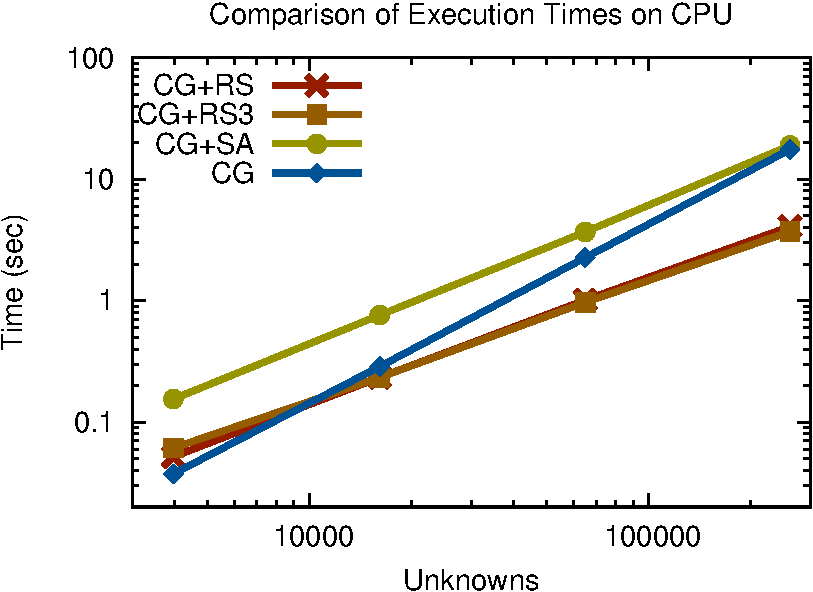
\includegraphics[width=0.7\textwidth]{figures/cpu_scaling-2}
  \end{center}
 \end{block}
   
\end{frame}

\begin{frame}[fragile]{Conjugate Gradient}

 \begin{block}{Implications}
   \begin{itemize}
   \item Kernel launches expensive
   \item Delicate balance for preconditioners
  \end{itemize}
  
    \vspace*{.8cm}
  \begin{center}
   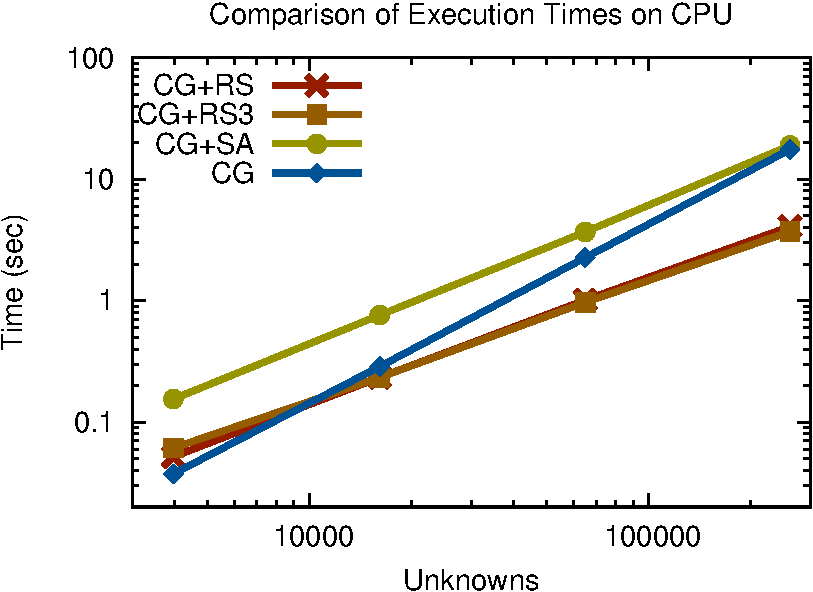
\includegraphics[width=0.48\textwidth]{figures/cpu_scaling-2} \hfill
   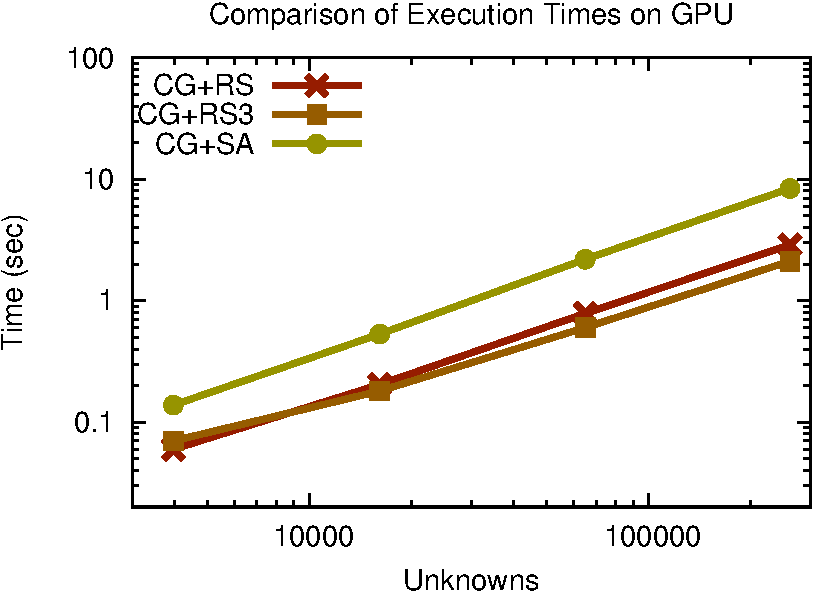
\includegraphics[width=0.48\textwidth]{figures/gpu_scaling-1}
  \end{center}
    \vspace*{.8cm}  
 \end{block}
   
\end{frame}

\begin{frame}[fragile]{Conjugate Gradient}

 \begin{block}{Implications}
   \begin{itemize}
   \item Kernel launches expensive
   \item Delicate balance for preconditioners
  \end{itemize}
  
      \vspace*{.8cm}
  \begin{center}
   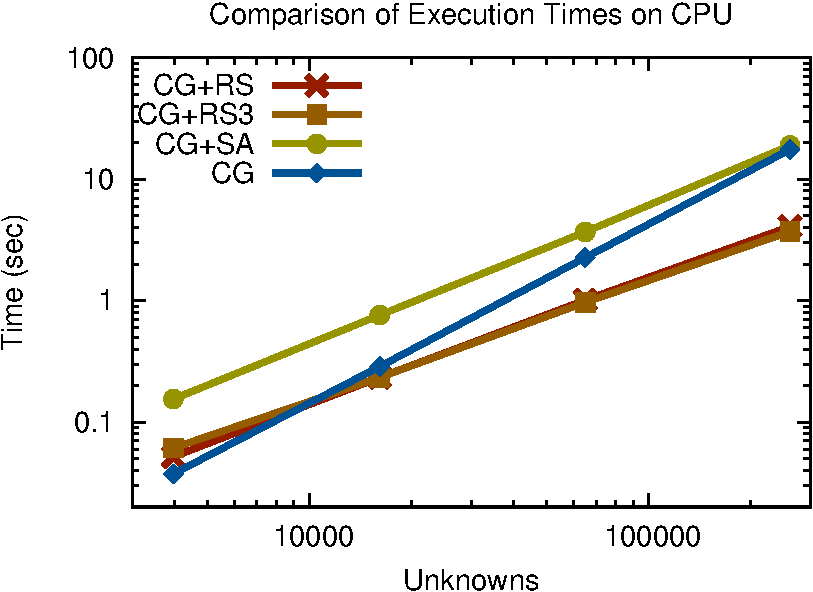
\includegraphics[width=0.48\textwidth]{figures/cpu_scaling-2} \hfill
   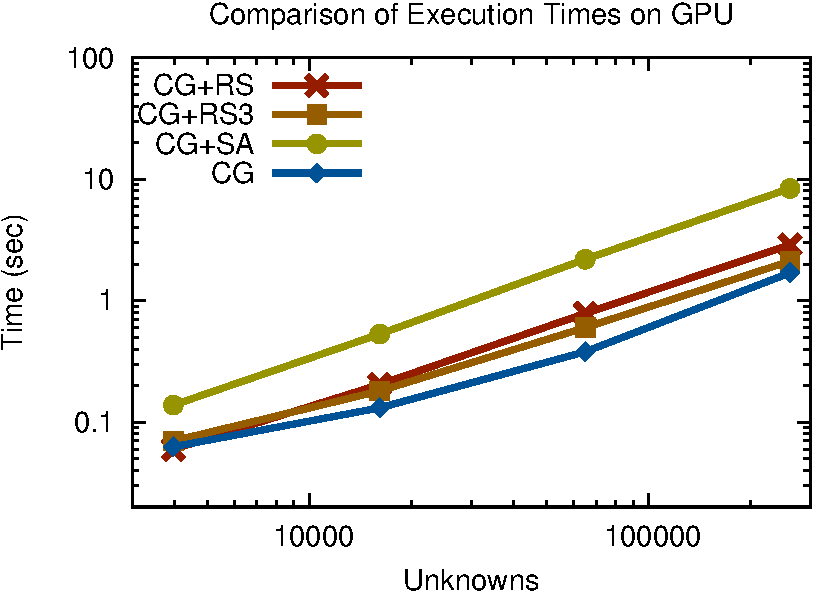
\includegraphics[width=0.48\textwidth]{figures/gpu_scaling-2}
  \end{center}
      \vspace*{.8cm}  
 \end{block}
   
\end{frame}


%%% CG optimizations:
% Step 1: CSR vs. ELL vs. HYB (to the extent possible)

\begin{frame}[fragile]{Conjugate Gradient Optimizations}

 \vspace*{2cm}
 \begin{block}{Optimization 1}
   \begin{itemize}
   \item Get best performance out of SpMV
   \item Compare different sparse matrix types
  \end{itemize}
 \end{block}

 \vspace*{2cm}
    {\small Cf.: N.~Bell: Implementing sparse matrix-vector multiplication\\ on throughput-oriented processors. \textit{Proc.~SC '09}}


\end{frame}

\begin{frame}[fragile]{Conjugate Gradients}
 \begin{block}{}
 \begin{center}
  \vspace*{-0.5cm}
  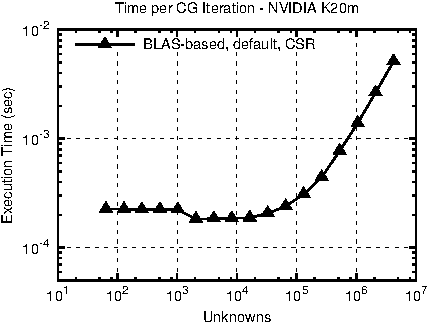
\includegraphics[width=0.85\textwidth]{figures/cg-k20m-0}
 \end{center}

 \begin{itemize}
  \item   \vspace*{-0.3cm} {\small (2D Finite Difference Discretization)}
 \end{itemize}
 \end{block}   
\end{frame}

\begin{frame}[fragile]{Conjugate Gradients}
 \begin{block}{}
 \begin{center}
  \vspace*{-0.5cm}
  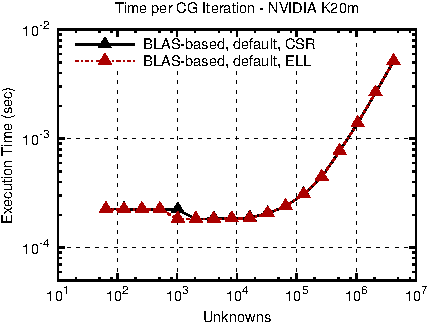
\includegraphics[width=0.85\textwidth]{figures/cg-k20m-1}
 \end{center}

 \begin{itemize}
  \item   \vspace*{-0.3cm} {\small (2D Finite Difference Discretization)}
 \end{itemize}
 \end{block}   
\end{frame}

\begin{frame}[fragile]{Conjugate Gradients}
 \begin{block}{}
 \begin{center}
  \vspace*{-0.5cm}
  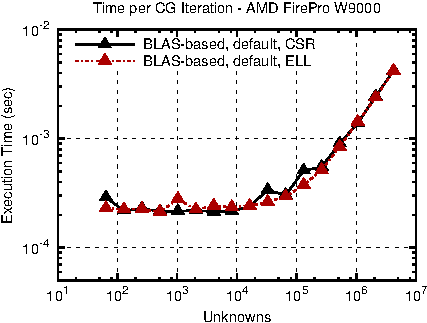
\includegraphics[width=0.85\textwidth]{figures/cg-firepro-w9000-1}
 \end{center}

 \begin{itemize}
  \item   \vspace*{-0.3cm} {\small (2D Finite Difference Discretization)}
 \end{itemize}
 \end{block}   
\end{frame}


% Step 2: Kernel parameters
\begin{frame}[fragile]{Conjugate Gradient Optimizations}

 \begin{block}{Optimization 2}
   \begin{itemize}
   \item Optimize kernel parameters for each operation
  \end{itemize}
 \end{block}
   
\end{frame}


\begin{frame}{Outline}
 \begin{center}
  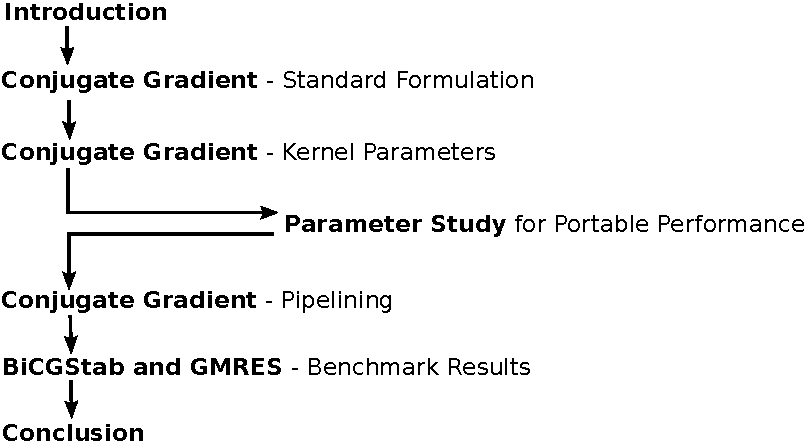
\includegraphics[width=0.9\textwidth]{figures/outline-crop}
 \end{center}
\end{frame}
